\renewcommand*\chappic{img/diff-crypt.pdf}
\renewcommand*\chapquote{Just because it's automatic doesn't mean it works.}
\renewcommand*\chapquotesrc{Daniel J. Bernstein}
%
\chapter{Differential cryptanalysis}
\label{ch:dc}
%
In chapter~\ref{ch:hash} we defined two hash functions. In this chapter
we consider such functions from a differential perspective. Differential
considerations will turn out to yield successful collision attacks on hash
functions. We introduce a notation to easily represent differential
characteristics.

\section{Motivation}
\label{sec:dc-motivation}
%
In August 2004, Wang et al. published results at Crypto'04~\cite{wang2004} which revealed
that MD4, MD5, HAVAL-128 and RIPEMD can be broken practically using differential cryptanalysis.
Their work is based on preliminary work by Hans Dobbertin~\cite{Dobbertin1998}.
On an IBM~P690 machine, an MD5 collision can be computed in about one hour using this approach.
Collisions for HAVAL-128, MD4 and RIPEMD were found as well. Patrick Stach's \texttt{md4coll.c}
program~\cite{md4coll} implements Wang's approach and can find MD4 collisions in few seconds
on my Thinkpad~x220 setup specified in \hyperref[app:setup]{Appendix~\ref{app:setup}}.

Let $n$ denote the digest size, i.e. the size of the hash value $h(x)$ in bits.
Due to the birthday paradox, a collision attack has a generic complexity of $2^{n/2}$
whereas preimage and second preimage attacks have generic complexities of $2^n$.
In other words it is computationally easier to find any two colliding hash values
than the preimage or second preimage for a given hash value.

Following results by Wang et al., differential cryptanalysis was shown as
powerful tool for cryptanalysis of hash algorithms. This thesis applies those
ideas to satisfiability approaches.

\begin{table}[bt]
  \begin{center}
    \begin{tabular}{cccc}
      \hline \hline
      \multicolumn{4}{c}{Message 1} \\
      \hline
      4d7a9c83 & \textbf{d6cb927a} & \textbf{29d5a578} & 57a7a5ee \\
      de748a3c & dcc366b3 & b683a020 & 3b2a5d9f \\
      c69d71b3 & f9e99198 & d79f805e & a63bb2e8 \\
      \textbf{45dc8e31} & 97e31fe5 & 2794bf08 & b9e8c3e9 \\
      \hline
      \multicolumn{4}{c}{Message 2} \\
      \hline
      4d7a9c83 & \textbf{56cb927a} & \textbf{b9d5a578} & 57a7a5ee \\
      de748a3c & dcc366b3 & b683a020 & 3b2a5d9f \\
      c69d71b3 & f9e99198 & d79f805e & a63bb2e8 \\
      \textbf{45dd8e31} & 97e31fe5 & 2794bf08 & b9e8c3e9 \\
      \hline
      \multicolumn{4}{c}{Hash value of Message 1 and Message 2} \\
      \hline
      5f5c1a0d & 71b36046 & 1b5435da & 9b0d807a \\
      \hline \hline
    \end{tabular}
    \caption[Hexadecimal values of one MD4 collisions given in paper~\cite{wang2004}]{
      One of two MD4 hash collisions provided in~\cite{wang2004}.
      Values are given in hexadecimal, message words are enumerated from
      left to right, top to bottom. Differences are highlighted in
      bold for illustration purposes. For comparison the first bits
      of Message 1 are \texttt{11000001\dots} and the last bits are
      \texttt{\dots10011101}.
      A message represents one block of 512~bits.
      %The hash value consists of 128~bits.
    }
    \label{tab:wang-md4-collision1}
  \end{center}
\end{table}

\newpage
\section{Fundamentals}
\label{sec:dc-fundamentals}
%
\index{Hash collision}
\begin{defi}[Hash collision]
  Given a hash function $h$,
  a hash collision is a pair $(x, x_2)$ with $x \neq x_2$ such that
  $h(x) = h(x_2)$.
\end{defi}

Differential cryptanalysis is based on the idea to consider two execution states
of hash algorithms for slightly different input messages. We trace those difference
to learn about the propagation of message differences.

TODO: explain pseudo collisions

Hash algorithms consume input values as blocks of bits.
As far as the length of the input must not conform to the block size,
padding is applied. Now consider such a block of input values
and another copy of it. We use those two blocks as inputs for two
hash algorithm implementations, but provide slight modifications in few bits.
MD4 has 48 round function applications in 3 rounds.
Differential cryptanalysis considers the difference in the evaluation
state between the two instances (compare with Figure~\ref{tab:collision-attack}).

Visualizing those differences helps the cryptanalyst to find modifications yielding
a small number of differences in the evaluation state.
The cryptanalyst consecutively modifies the input values to eventually
receive a collision in the output value.
If the number of differences in the evaluation state is small,
this trail is expected to result in a hash collision with higher probability.

\begin{figure}[pbt]
  \begin{center}
    \fbox{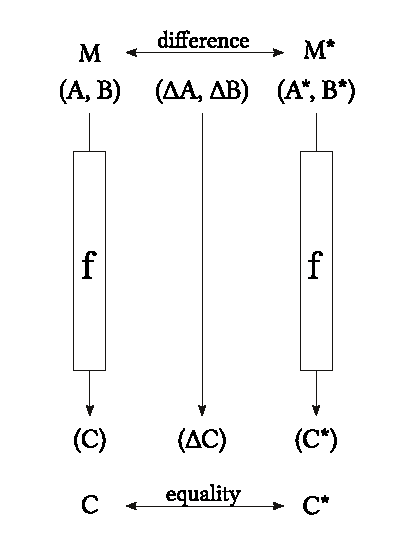
\includegraphics[width=0.55\textwidth]{img/diff_cryptanalysis.pdf}}
    \caption[Typical attack setting for a collision attack]{
      Typical attack setting for a collision attack:
      Hash function $f$ is applied to two inputs $M$ and $M^*$ which differ
      by some predefined bits. $\triangle M$ describes the difference between
      these values. A hash collision is given if and only if output values
      $C$ and $C^*$ show the same value. In differential cryptanalysis we observe
      the differences between two instances applying function $f$
      to inputs $M$ and $M^*$.
    }
    \label{tab:collision-attack}
  \end{center}
\end{figure}

\section{Differential notation}
\label{sec:dc-notation}
%
\index{Bit condition}
\index{Generalized bit condition}
\index{Differential notation}
Differential notation helps us to visualize differential characteristics
by defining so-called \emph{generalized bit conditions}.
It was introduced by Christian Rechberger and Christophe de Canni\`ere
in 2006~\cite[Section 3.2]{char-2006}, inspired by \emph{signed differences} by
Wang~et al. and is shown in Table~\ref{tab:diff-notation}.

Consider two hash algorithm implementations. Let $x_i$ be some bit
from the first implementation and let $x_i^*$ be the corresponding bit
from the second implementation. Differences are computed using a \boolf{XOR}
and commonly denoted as $\Delta x = x_i \oplus x_i^*$.
Bit conditions allow us to encode possible
relations between bits $x_i$ and $x_i^*$.

For example, let us take a look at the original Wang et al. hash collision
in MD4 provided in Table~\ref{tab:wang-md4-collision1}.
We extract all values with differences and represent them using differential notation.
This gives us Table~\ref{tab:differential-wang-values}.

The following properties hold for bit conditions:
\begin{itemize}[noitemsep,topsep=0pt]
  \item If $x_i = x_i^*$ holds and some value is known, $\set{0,1}$ contains its bit condition.
  \item If $x_i \neq x_i^*$ holds and some value is known, $\set{u,n}$ contains its bit condition.
  \item If $x_i = x_i^*$ holds and the values are unknown, its bit condition is $\dnI{-}$.
  \item If $x_i \neq x_i^*$ holds and the values are unknown, its bit condition is $\dnI{x}$.
\end{itemize}
Applying this notation to hash collisions means that arbitrary bit conditions
(expect for \dnI{\#}) can be specified for the input values. In one of the
intermediate iterations, we enforce a difference using one of the bit conditions
$\set{u,n,x}$. This excludes trivial solutions with no differences from the set of
possible solutions. And the final values need to lack differences thus are
represented using \dnI{-}.

\begin{table}[bt]
  \begin{center}
    \small
    \begin{tabular}{lll}
      \hline \hline
      bit & binary & hexadecimal representation / differential notation \\
      \hline \hline
      $x_0$ & \dnI{d6cb927a} & \dnI{11010110110010111001001001111010} \\
      $x_1$ & \dnI{29d5a578} & \dnI{00101001110101011010010101111000} \\
      $x_2$ & \dnI{45dc8e31} & \dnI{01000101110111001000111000110001} \\
      \hline
      $x_0^*$ & \dnI{56cb927a} & \dnI{01010110110010111001001001111010} \\
      $x_1^*$ & \dnI{b9d5a578} & \dnI{10111001110101011010010101111000} \\
      $x_2^*$ & \dnI{45dd8e31} & \dnI{01000101110111011000111000110001} \\
      \hline
      $\Delta x$ & & \dnI{u1010110110010111001001001111010} \\
                 & & \dnI{n01n1001110101011010010101111000} \\
                 & & \dnI{010001011101110n1000111000110001} \\
      \hline \hline
    \end{tabular}
    \caption[Bit differences in the original Wang et al. hash collision]{
      The three words different between Message~1 and Message~2 of the original
      MD4 hash collision. The last three lines show how differences can be
      written down using bit conditions. As far as 4 symbols are not from the
      set $\set{0, 1}$ it holds that the messages differ by 4~bits.
    }
    \label{tab:differential-wang-values}
  \end{center}
\end{table}

\begin{table}[b]
  \small
  \begin{center}
    \begin{tabular}{|c|cccc|}
    \hline\hline
      $(x_i, x_i^*)$ & $(0,0)$ & $(1,0)$ & $(0,1)$ & $(1,1)$ \\
    \hline
      \dnI{?}        & \yes    & \yes    & \yes    & \yes    \\
      \dnI{-}        & \yes    & \no     & \no     & \yes    \\
      \dnI{x}        & \no     & \yes    & \yes    & \no     \\
      \dnI{0}        & \yes    & \no     & \no     & \no     \\
      \dnI{u}        & \no     & \yes    & \no     & \no     \\
      \dnI{n}        & \no     & \no     & \yes    & \no     \\
      \dnI{1}        & \no     & \no     & \no     & \yes    \\
      \dnI{\#}       & \no     & \no     & \no     & \no     \\
    \hline \hline
    \end{tabular}
    \begin{tabular}{|c|cccc|}
    \hline\hline
      $(x_i, x_i^*)$ & $(0,0)$ & $(1,0)$ & $(0,1)$ & $(1,1)$ \\
    \hline
      \dnI{3}        & \yes    & \yes    & \no     & \no     \\
      \dnI{5}        & \yes    & \no     & \yes    & \no     \\
      \dnI{7}        & \yes    & \yes    & \yes    & \no     \\
      \dnI{A}        & \no     & \yes    & \no     & \yes    \\
      \dnI{B}        & \yes    & \yes    & \no     & \yes    \\
      \dnI{C}        & \no     & \no     & \yes    & \yes    \\
      \dnI{D}        & \yes    & \no     & \yes    & \yes    \\
      \dnI{E}        & \no     & \yes    & \yes    & \yes    \\
    \hline \hline
    \end{tabular}
    \caption{
      Differential notation as introduced in~\cite{char-2006}.
      The left-most column specifies a symbol called \enquote{bit condition}
      and right-side columns indicate which bit configurations
      are possible for two given bits $x_i$ and $x_i^*$.
    }
    \label{tab:diff-notation}
  \end{center}
\end{table}

\begin{table}[b]
  \begin{center}
    \begin{tabular}{cp{5cm}cl}
      $\Delta x$      & conjunctive normal form &
      $\Delta x$      & conjunctive normal form \\
    \hline
      \dnI{\#}        & $(x) \land (\neg x)$ &
      \dnI{1}         & $(x) \land (x^*)$ \\

      \dnI{0}         & $(\neg x) \land (\neg x^*)$ &
      \dnI{-}         & $\neg (x \oplus x^*)$ \\

      \dnI{u}         & $(x) \land (\neg x^*)$ &
      \dnI{A}         & $(x)$ \\

      \dnI{3}         & $(\neg x^*)$ &
      \dnI{B}         & $(x \lor \neg x^*)$ \\

      \dnI{n}         & $(\neg x) \land (x^*)$ &
      \dnI{C}         & $(x^*)$ \\

      \dnI{5}         & $(\neg x)$ &
      \dnI{D}         & $(\neg x \lor x^*)$ \\

      \dnI{x}         & $(x \oplus x^*)$ &
      \dnI{E}         & $(x \lor x^*)$ \\

      \dnI{7}         & $(\neg x \lor \neg x^*)$ &
      \dnI{?}         &  \\
    \end{tabular}
    \caption[Representation of bit conditions as CNF]{
      All bit conditions represented as CNF using
      two boolean variables $x$ and $x^*$ to represent
      two bits.
    }
    \label{tab:simple-eval-clauses}
  \end{center}
\end{table}


\section{A simple addition example}
\label{sec:dc-example}
%
TODO:
\begin{itemize}
  \item illustrate how differences propagate by an addition example illustrated in differential notation
  \item reference to Magnus Daum's thesis ($\neq$ signed bit diff desc)
\end{itemize}

\section{Differential path}
\label{sec:dc-path}
%
TODO:
\begin{itemize}
  \item refer to some testcase which shows a differential path with many unresolved differences.
  \item Then show the corresponding testcase where \dnI{?} became \dnI{-} and \dnI{x}.
  \item Illustrate how MD4 and SHA-256 descriptions maps to matrix representation.
\end{itemize}
